\documentclass[border=10pt]{standalone}
\usepackage[svgnames]{xcolor}
\usepackage{amsmath}
\usepackage{pgfplots}
\pgfplotsset{compat=newest}
\usepackage[sfdefault]{FiraSans}
\usepackage{FiraMono}
\renewcommand*\familydefault{\sfdefault}
\begin{document}
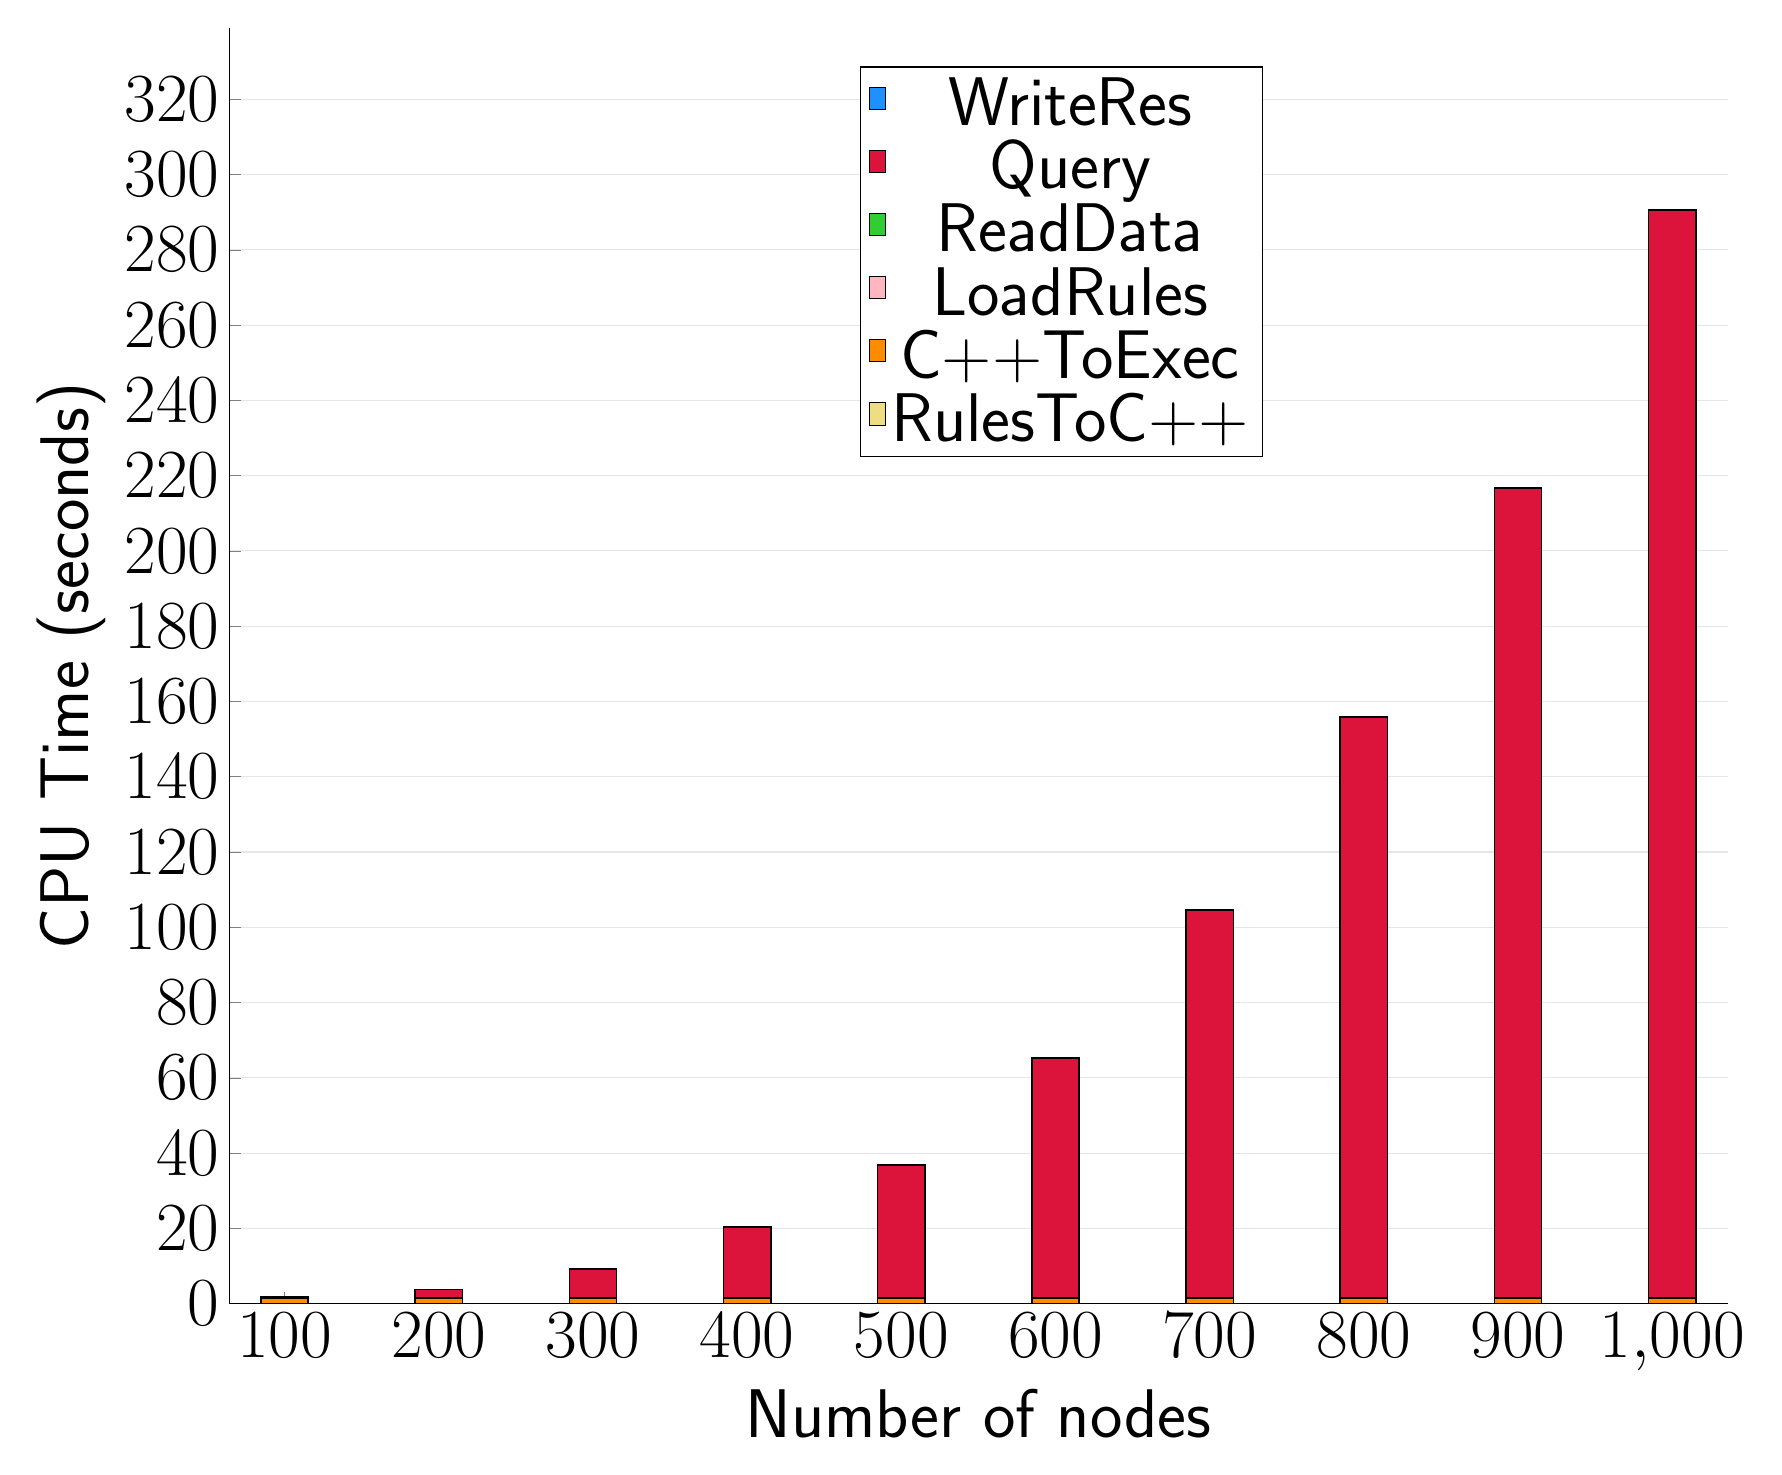
\begin{tikzpicture}
\begin{axis}[
   ybar stacked,
   width=1.7\textwidth,
   bar width=0.6cm,
   ymajorgrids, tick align=inside,
   major grid style={draw=gray!20},
   xtick=data,
   ymin=0, ymax=338.8692,
   axis x line*=bottom,
   axis y line*=left,
   enlarge x limits=0.04,
   legend style={
       at={(0.69, 0.97)},
       anchor=north east,
       legend columns=1,
       font=\Huge,
   },
   ylabel={CPU Time (seconds)},
   xlabel={Number of nodes},
   label style={font=\Huge},
   tick label style={font=\Huge},
]
\addlegendimage{fill=DodgerBlue, draw=black, line width=0.2pt}
\addlegendentry{WriteRes}
\addlegendimage{fill=Crimson, draw=black, line width=0.2pt}
\addlegendentry{Query}
\addlegendimage{fill=LimeGreen, draw=black, line width=0.2pt}
\addlegendentry{ReadData}
\addlegendimage{fill=LightPink, draw=black, line width=0.2pt}
\addlegendentry{LoadRules}
\addlegendimage{fill=DarkOrange, draw=black, line width=0.2pt}
\addlegendentry{C++ToExec}
\addlegendimage{fill=LightGoldenrod, draw=black, line width=0.2pt}
\addlegendentry{RulesToC++}
\addplot +[fill=LightGoldenrod, draw=black, line width=0.55pt] coordinates {
(100, 0.0020000000000000005)
(200, 0.0020000000000000005)
(300, 0.007999999999999997)
(400, 0.0020000000000000005)
(500, 0.0020000000000000005)
(600, 0.0020000000000000005)
(700, 0.0)
(800, 0.004000000000000001)
(900, 0.0)
(1000, 0.0)
};
\addplot +[fill=DarkOrange, draw=black, line width=0.55pt] coordinates {
(100, 1.482)
(200, 1.482)
(300, 1.48)
(400, 1.48)
(500, 1.482)
(600, 1.486)
(700, 1.472)
(800, 1.47)
(900, 1.4780000000000002)
(1000, 1.502)
};
\addplot +[fill=LightPink, draw=black, line width=0.55pt] coordinates {
(100, 0.0001818)
(200, 0.00017740000000000003)
(300, 0.00018700000000000002)
(400, 0.00018899999999999999)
(500, 0.00020800000000000001)
(600, 0.00020740000000000003)
(700, 0.0001186)
(800, 0.0001024)
(900, 0.00023579999999999999)
(1000, 0.00018680000000000001)
};
\addplot +[fill=LimeGreen, draw=black, line width=0.55pt] coordinates {
(100, 0.000792)
(200, 0.0011237999999999999)
(300, 0.0014081999999999999)
(400, 0.0020178)
(500, 0.0024934)
(600, 0.003045)
(700, 0.0023056)
(800, 0.0019614)
(900, 0.0046672)
(1000, 0.0032714)
};
\addplot +[fill=Crimson, draw=black, line width=0.55pt] coordinates {
(100, 0.3054582)
(200, 2.297596)
(300, 7.766288)
(400, 18.82078)
(500, 35.3274)
(600, 63.66976)
(700, 103.03400000000002)
(800, 154.2942)
(900, 215.1904)
(1000, 288.8692)
};
\addplot +[fill=DodgerBlue, draw=black, line width=0.55pt] coordinates {
(100, 0.002468)
(200, 0.0089116)
(300, 0.0195672)
(400, 0.034351200000000005)
(500, 0.0533714)
(600, 0.07718799999999999)
(700, 0.1043056)
(800, 0.1356366)
(900, 0.17171799999999998)
(1000, 0.2105976)
};
\end{axis}
\end{tikzpicture}

\end{document}
